\chapter{完整搜索}

\key{完整搜索}是一种通用方法，
可以用来解决几乎任何算法问题。
其基本思想是用暴力方法生成问题的
所有可能的解，
然后根据问题的要求选择最优解或统计
解的数量。

如果有足够的时间遍历所有解，
那么完整搜索是一种很好的技术，
因为搜索通常容易实现，
而且总是能给出正确答案。
如果完整搜索太慢，
则可能需要其他技术，例如贪心算法或
动态规划。

\section{生成子集}

\index{子集}

我们首先考虑生成一个包含$n$个元素的集合的
所有子集的问题。
例如，$\{0,1,2\}$的子集有
$\emptyset$、$\{0\}$、$\{1\}$、$\{2\}$、$\{0,1\}$、
$\{0,2\}$、$\{1,2\}$和$\{0,1,2\}$。
生成子集有两种常用方法：
我们可以执行递归搜索，
也可以利用整数的位表示。

\subsubsection{方法1}

遍历一个集合的所有子集的一种优雅方式
是使用递归。
以下函数\texttt{search}
生成集合$\{0,1,\ldots,n-1\}$的子集。
该函数维护一个向量\texttt{subset}，
用于存储每个子集的元素。
当函数以参数0调用时，搜索开始。

\begin{lstlisting}
void search(int k) {
    if (k == n) {
        // 处理子集
    } else {
        search(k+1);
        subset.push_back(k);
        search(k+1);
        subset.pop_back();
    }
}
\end{lstlisting}

当函数\texttt{search}
以参数$k$调用时，
它决定是否将元素$k$
包含在子集中，
在两种情况下，
都以参数$k+1$调用自身。
然而，如果$k=n$，函数会发现
所有元素都已被处理，
一个子集已经生成。

下面的树展示了$n=3$时的函数调用过程。
我们总是可以选择左分支
（$k$不包含在子集中）或右分支
（$k$包含在子集中）。

\begin{center}
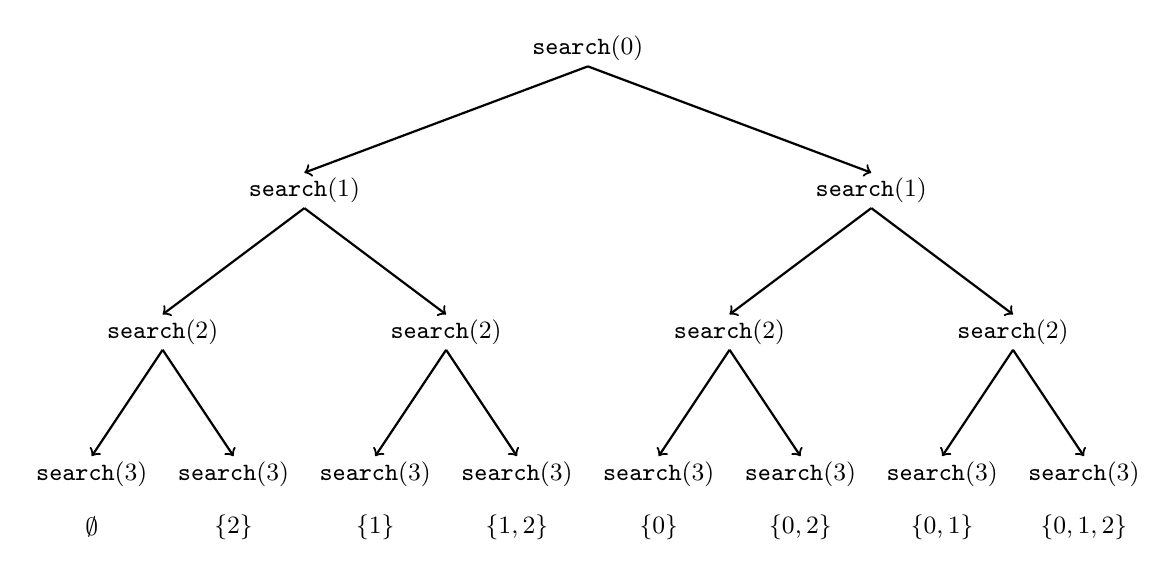
\begin{tikzpicture}[scale=.45]
  \begin{scope}
    \small
    \node at (0,0) {$\texttt{search}(0)$};

    \node at (-8,-4) {$\texttt{search}(1)$};
    \node at (8,-4) {$\texttt{search}(1)$};

    \path[draw,thick,->] (0,0-0.5) -- (-8,-4+0.5);
    \path[draw,thick,->] (0,0-0.5) -- (8,-4+0.5);

    \node at (-12,-8) {$\texttt{search}(2)$};
    \node at (-4,-8) {$\texttt{search}(2)$};
    \node at (4,-8) {$\texttt{search}(2)$};
    \node at (12,-8) {$\texttt{search}(2)$};

    \path[draw,thick,->] (-8,-4-0.5) -- (-12,-8+0.5);
    \path[draw,thick,->] (-8,-4-0.5) -- (-4,-8+0.5);
    \path[draw,thick,->] (8,-4-0.5) -- (4,-8+0.5);
    \path[draw,thick,->] (8,-4-0.5) -- (12,-8+0.5);

    \node at (-14,-12) {$\texttt{search}(3)$};
    \node at (-10,-12) {$\texttt{search}(3)$};
    \node at (-6,-12) {$\texttt{search}(3)$};
    \node at (-2,-12) {$\texttt{search}(3)$};
    \node at (2,-12) {$\texttt{search}(3)$};
    \node at (6,-12) {$\texttt{search}(3)$};
    \node at (10,-12) {$\texttt{search}(3)$};
    \node at (14,-12) {$\texttt{search}(3)$};

    \node at (-14,-13.5) {$\emptyset$};
    \node at (-10,-13.5) {$\{2\}$};
    \node at (-6,-13.5) {$\{1\}$};
    \node at (-2,-13.5) {$\{1,2\}$};
    \node at (2,-13.5) {$\{0\}$};
    \node at (6,-13.5) {$\{0,2\}$};
    \node at (10,-13.5) {$\{0,1\}$};
    \node at (14,-13.5) {$\{0,1,2\}$};


    \path[draw,thick,->] (-12,-8-0.5) -- (-14,-12+0.5);
    \path[draw,thick,->] (-12,-8-0.5) -- (-10,-12+0.5);
    \path[draw,thick,->] (-4,-8-0.5) -- (-6,-12+0.5);
    \path[draw,thick,->] (-4,-8-0.5) -- (-2,-12+0.5);
    \path[draw,thick,->] (4,-8-0.5) -- (2,-12+0.5);
    \path[draw,thick,->] (4,-8-0.5) -- (6,-12+0.5);
    \path[draw,thick,->] (12,-8-0.5) -- (10,-12+0.5);
    \path[draw,thick,->] (12,-8-0.5) -- (14,-12+0.5);
\end{scope}
\end{tikzpicture}
\end{center}

\subsubsection{方法2}

另一种生成子集的方法基于
整数的位表示。
一个包含$n$个元素的集合的每个子集
都可以表示为一个$n$位的序列，
对应于$0 \ldots 2^n-1$之间的一个整数。
位序列中的1表示
哪些元素包含在子集中。

通常的约定是，
最后一位对应元素0，
倒数第二位对应元素1，
以此类推。
例如，25的位表示
是11001，对应子集$\{0,3,4\}$。

以下代码遍历包含$n$个元素的集合的
所有子集

\begin{lstlisting}
for (int b = 0; b < (1<<n); b++) {
    // 处理子集
}
\end{lstlisting}

以下代码展示了如何找出
与某个位序列对应的子集的元素。
在处理每个子集时，
代码构建一个包含该子集中
元素的向量。

\begin{lstlisting}
for (int b = 0; b < (1<<n); b++) {
    vector<int> subset;
    for (int i = 0; i < n; i++) {
        if (b&(1<<i)) subset.push_back(i);
    }
}
\end{lstlisting}

\section{生成排列}

\index{排列}

接下来我们考虑生成一个包含$n$个元素的集合的
所有排列的问题。
例如，$\{0,1,2\}$的排列有
$(0,1,2)$、$(0,2,1)$、$(1,0,2)$、$(1,2,0)$、
$(2,0,1)$和$(2,1,0)$。
同样有两种方法：
我们可以使用递归，也可以
迭代地遍历排列。

\subsubsection{方法1}

与子集类似，排列也可以使用递归来生成。
以下函数\texttt{search}遍历集合$\{0,1,\ldots,n-1\}$的所有排列。
该函数构建一个向量\texttt{permutation}
来存储排列，
当函数不带参数调用时搜索开始。

\begin{lstlisting}
void search() {
    if (permutation.size() == n) {
        // 处理排列
    } else {
        for (int i = 0; i < n; i++) {
            if (chosen[i]) continue;
            chosen[i] = true;
            permutation.push_back(i);
            search();
            chosen[i] = false;
            permutation.pop_back();
        }
    }
}
\end{lstlisting}

每次函数调用都会向\texttt{permutation}
中添加一个新元素。
数组\texttt{chosen}指示哪些
元素已经包含在排列中。
如果\texttt{permutation}的大小等于集合的大小，
则一个排列已经生成。

\subsubsection{方法2}

\index{next\_permutation@\texttt{next\_permutation}}

另一种生成排列的方法是
从排列$\{0,1,\ldots,n-1\}$开始，
重复使用一个函数来构造递增顺序的
下一个排列。
C++标准库中包含函数
\texttt{next\_permutation}，可以用于此目的：

\begin{lstlisting}
vector<int> permutation;
for (int i = 0; i < n; i++) {
    permutation.push_back(i);
}
do {
    // 处理排列
} while (next_permutation(permutation.begin(),permutation.end()));
\end{lstlisting}

\section{回溯}

\index{回溯}

\key{回溯}算法
从一个空解开始，
逐步扩展解。
搜索过程递归地遍历
构造解的所有不同方式。

\index{皇后问题}

作为一个例子，考虑计算在$n \times n$棋盘上放置$n$个皇后
使得没有两个皇后互相攻击的
方法数量的问题。
例如，当$n=4$时，
有两个可能的解：

\begin{center}
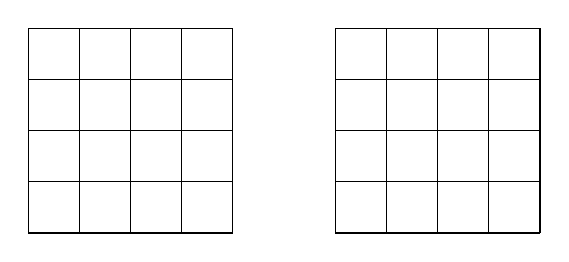
\begin{tikzpicture}[scale=.65]
  \begin{scope}
    \draw (0, 0) grid (4, 4);
    \node at (1.5,3.5) {\symqueen};
    \node at (3.5,2.5) {\symqueen};
    \node at (0.5,1.5) {\symqueen};
    \node at (2.5,0.5) {\symqueen};

    \draw (6, 0) grid (10, 4);
    \node at (6+2.5,3.5) {\symqueen};
    \node at (6+0.5,2.5) {\symqueen};
    \node at (6+3.5,1.5) {\symqueen};
    \node at (6+1.5,0.5) {\symqueen};

  \end{scope}
\end{tikzpicture}
\end{center}

这个问题可以用回溯法解决，
方法是逐行将皇后放置到棋盘上。
更准确地说，每一行恰好放置
一个皇后，使得没有皇后攻击
之前放置的任何皇后。
当所有$n$个皇后都放置到棋盘上时，
就找到了一个解。

例如，当$n=4$时，
回溯算法生成的一些部分解如下：

\begin{center}
\begin{tikzpicture}[scale=.55]
  \begin{scope}
    \draw (0, 0) grid (4, 4);

    \draw (-9, -6) grid (-5, -2);
    \draw (-3, -6) grid (1, -2);
    \draw (3, -6) grid (7, -2);
    \draw (9, -6) grid (13, -2);

    \node at (-9+0.5,-3+0.5) {\symqueen};
    \node at (-3+1+0.5,-3+0.5) {\symqueen};
    \node at (3+2+0.5,-3+0.5) {\symqueen};
    \node at (9+3+0.5,-3+0.5) {\symqueen};

    \draw (2,0) -- (-7,-2);
    \draw (2,0) -- (-1,-2);
    \draw (2,0) -- (5,-2);
    \draw (2,0) -- (11,-2);

    \draw (-11, -12) grid (-7, -8);
    \draw (-6, -12) grid (-2, -8);
    \draw (-1, -12) grid (3, -8);
    \draw (4, -12) grid (8, -8);
    \draw[white] (11, -12) grid (15, -8);
    \node at (-11+1+0.5,-9+0.5) {\symqueen};
    \node at (-6+1+0.5,-9+0.5) {\symqueen};
    \node at (-1+1+0.5,-9+0.5) {\symqueen};
    \node at (4+1+0.5,-9+0.5) {\symqueen};
    \node at (-11+0+0.5,-10+0.5) {\symqueen};
    \node at (-6+1+0.5,-10+0.5) {\symqueen};
    \node at (-1+2+0.5,-10+0.5) {\symqueen};
    \node at (4+3+0.5,-10+0.5) {\symqueen};

    \draw (-1,-6) -- (-9,-8);
    \draw (-1,-6) -- (-4,-8);
    \draw (-1,-6) -- (1,-8);
    \draw (-1,-6) -- (6,-8);

    \node at (-9,-13) {非法};
    \node at (-4,-13) {非法};
    \node at (1,-13) {非法};
    \node at (6,-13) {合法};

  \end{scope}
\end{tikzpicture}
\end{center}

在最底层，前三个配置
是非法的，因为皇后之间互相攻击。
然而，第四个配置是合法的，
通过再放置两个皇后到棋盘上，
它可以扩展为一个完整的解。
只有一种方法来放置剩余的两个皇后。

\begin{samepage}
该算法可以按如下方式实现：
\begin{lstlisting}
void search(int y) {
    if (y == n) {
        count++;
        return;
    }
    for (int x = 0; x < n; x++) {
        if (column[x] || diag1[x+y] || diag2[x-y+n-1]) continue;
        column[x] = diag1[x+y] = diag2[x-y+n-1] = 1;
        search(y+1);
        column[x] = diag1[x+y] = diag2[x-y+n-1] = 0;
    }
}
\end{lstlisting}
\end{samepage}
搜索从调用\texttt{search(0)}开始。
棋盘的大小为$n \times n$，
代码将解的数量计算到
\texttt{count}中。

代码假设棋盘的行和列
从0编号到$n-1$。
当函数\texttt{search}
以参数$y$调用时，
它在第$y$行放置一个皇后，
然后以参数$y+1$调用自身。
如果$y=n$，则找到一个解，
变量\texttt{count}增加一。

数组\texttt{column}记录包含皇后的列，
数组\texttt{diag1}和\texttt{diag2}
记录对角线。
不允许向已经包含皇后的列或对角线上
再添加另一个皇后。
例如，$4 \times 4$棋盘的列和对角线的
编号如下：

\begin{center}
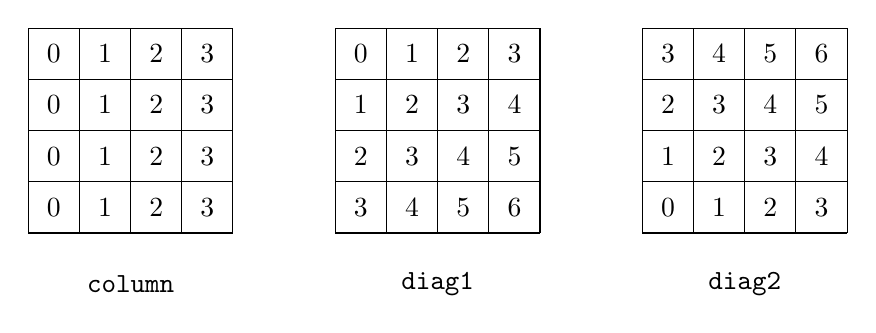
\begin{tikzpicture}[scale=.65]
  \begin{scope}
    \draw (0-6, 0) grid (4-6, 4);
    \node at (-6+0.5,3.5) {$0$};
    \node at (-6+1.5,3.5) {$1$};
    \node at (-6+2.5,3.5) {$2$};
    \node at (-6+3.5,3.5) {$3$};
    \node at (-6+0.5,2.5) {$0$};
    \node at (-6+1.5,2.5) {$1$};
    \node at (-6+2.5,2.5) {$2$};
    \node at (-6+3.5,2.5) {$3$};
    \node at (-6+0.5,1.5) {$0$};
    \node at (-6+1.5,1.5) {$1$};
    \node at (-6+2.5,1.5) {$2$};
    \node at (-6+3.5,1.5) {$3$};
    \node at (-6+0.5,0.5) {$0$};
    \node at (-6+1.5,0.5) {$1$};
    \node at (-6+2.5,0.5) {$2$};
    \node at (-6+3.5,0.5) {$3$};

    \draw (0, 0) grid (4, 4);
    \node at (0.5,3.5) {$0$};
    \node at (1.5,3.5) {$1$};
    \node at (2.5,3.5) {$2$};
    \node at (3.5,3.5) {$3$};
    \node at (0.5,2.5) {$1$};
    \node at (1.5,2.5) {$2$};
    \node at (2.5,2.5) {$3$};
    \node at (3.5,2.5) {$4$};
    \node at (0.5,1.5) {$2$};
    \node at (1.5,1.5) {$3$};
    \node at (2.5,1.5) {$4$};
    \node at (3.5,1.5) {$5$};
    \node at (0.5,0.5) {$3$};
    \node at (1.5,0.5) {$4$};
    \node at (2.5,0.5) {$5$};
    \node at (3.5,0.5) {$6$};

    \draw (6, 0) grid (10, 4);
    \node at (6.5,3.5) {$3$};
    \node at (7.5,3.5) {$4$};
    \node at (8.5,3.5) {$5$};
    \node at (9.5,3.5) {$6$};
    \node at (6.5,2.5) {$2$};
    \node at (7.5,2.5) {$3$};
    \node at (8.5,2.5) {$4$};
    \node at (9.5,2.5) {$5$};
    \node at (6.5,1.5) {$1$};
    \node at (7.5,1.5) {$2$};
    \node at (8.5,1.5) {$3$};
    \node at (9.5,1.5) {$4$};
    \node at (6.5,0.5) {$0$};
    \node at (7.5,0.5) {$1$};
    \node at (8.5,0.5) {$2$};
    \node at (9.5,0.5) {$3$};

    \node at (-4,-1) {\texttt{column}};
    \node at (2,-1) {\texttt{diag1}};
    \node at (8,-1) {\texttt{diag2}};

  \end{scope}
\end{tikzpicture}
\end{center}

令$q(n)$表示在$n \times n$棋盘上
放置$n$个皇后的方法数量。
上述回溯算法告诉我们，
例如$q(8)=92$。
当$n$增大时，搜索很快变慢，
因为解的数量呈指数级增长。
例如，使用上述算法计算$q(16)=14772512$
在现代计算机上已经大约需要一分钟\footnote{目前没有已知的方法可以高效地
计算更大的$q(n)$值。当前记录是
$q(27)=234907967154122528$，于2016年计算得出 \cite{q27}。}。

\section{搜索剪枝}

我们通常可以通过对搜索树剪枝来
优化回溯算法。
其思想是为算法添加“智能”，
使其尽快发现
一个部分解是否无法扩展
为完整的解。
这种优化可以对搜索效率
产生巨大的影响。

让我们考虑一个问题：
计算在$n \times n$网格中从左上角
到右下角且每个方格恰好访问一次的
路径数量。
例如，在$7 \times 7$网格中，
有111712条这样的路径。
其中一条路径如下：

\begin{center}
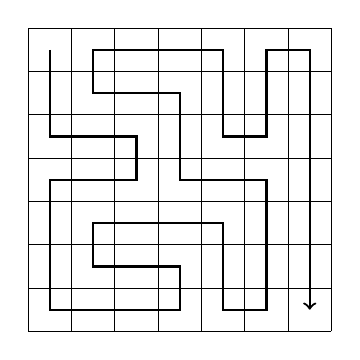
\begin{tikzpicture}[scale=.55]
  \begin{scope}
    \draw (0, 0) grid (7, 7);
    \draw[thick,->] (0.5,6.5) -- (0.5,4.5) -- (2.5,4.5) --
          (2.5,3.5) -- (0.5,3.5) -- (0.5,0.5) --
          (3.5,0.5) -- (3.5,1.5) -- (1.5,1.5) --
          (1.5,2.5) -- (4.5,2.5) -- (4.5,0.5) --
          (5.5,0.5) -- (5.5,3.5) -- (3.5,3.5) --
          (3.5,5.5) -- (1.5,5.5) -- (1.5,6.5) --
          (4.5,6.5) -- (4.5,4.5) -- (5.5,4.5) --
          (5.5,6.5) -- (6.5,6.5) -- (6.5,0.5);
  \end{scope}
\end{tikzpicture}
\end{center}

我们重点关注$7 \times 7$的情况，
因为其难度级别适合我们的需要。
我们从一个简单的回溯算法开始，
然后通过观察如何剪枝搜索
来逐步优化它。
在每次优化之后，我们测量算法的运行时间
和递归调用的次数，
以便清楚地看到每次优化
对搜索效率的影响。

\subsubsection{基本算法}

算法的第一个版本不包含
任何优化。我们简单地使用回溯来生成
从左上角到右下角的所有可能路径，
并统计这样的路径数量。

\begin{itemize}
\item
运行时间：483秒
\item
递归调用次数：760亿次
\end{itemize}

\subsubsection{优化1}

在任何解中，我们首先向下或向右
移动一步。
在第一步之后，总是有两条路径
关于网格的对角线对称。
例如，以下路径是对称的：

\begin{center}
\begin{tabular}{ccc}
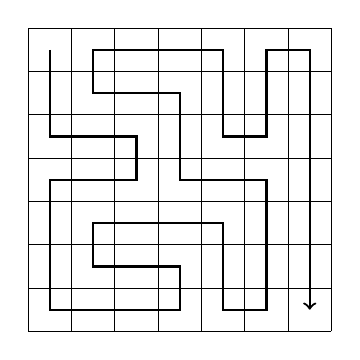
\begin{tikzpicture}[scale=.55]
  \begin{scope}
    \draw (0, 0) grid (7, 7);
    \draw[thick,->] (0.5,6.5) -- (0.5,4.5) -- (2.5,4.5) --
          (2.5,3.5) -- (0.5,3.5) -- (0.5,0.5) --
          (3.5,0.5) -- (3.5,1.5) -- (1.5,1.5) --
          (1.5,2.5) -- (4.5,2.5) -- (4.5,0.5) --
          (5.5,0.5) -- (5.5,3.5) -- (3.5,3.5) --
          (3.5,5.5) -- (1.5,5.5) -- (1.5,6.5) --
          (4.5,6.5) -- (4.5,4.5) -- (5.5,4.5) --
          (5.5,6.5) -- (6.5,6.5) -- (6.5,0.5);
  \end{scope}
\end{tikzpicture}
& \hspace{20pt}
& 
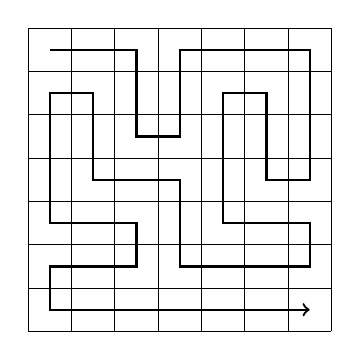
\begin{tikzpicture}[scale=.55]
  \begin{scope}[yscale=1,xscale=-1,rotate=-90]
    \draw (0, 0) grid (7, 7);
    \draw[thick,->] (0.5,6.5) -- (0.5,4.5) -- (2.5,4.5) --
          (2.5,3.5) -- (0.5,3.5) -- (0.5,0.5) --
          (3.5,0.5) -- (3.5,1.5) -- (1.5,1.5) --
          (1.5,2.5) -- (4.5,2.5) -- (4.5,0.5) --
          (5.5,0.5) -- (5.5,3.5) -- (3.5,3.5) --
          (3.5,5.5) -- (1.5,5.5) -- (1.5,6.5) --
          (4.5,6.5) -- (4.5,4.5) -- (5.5,4.5) --
          (5.5,6.5) -- (6.5,6.5) -- (6.5,0.5);
  \end{scope}
\end{tikzpicture}
\end{tabular}
\end{center}

因此，我们可以决定总是先
向下（或向右）移动一步，
最后将解的数量乘以二。

\begin{itemize}
\item
运行时间：244秒
\item
递归调用次数：380亿次
\end{itemize}

\subsubsection{优化2}

如果路径在访问网格中所有其他方格之前
就到达了右下角的方格，
显然不可能完成这个解。
以下路径就是一个例子：

\begin{center}
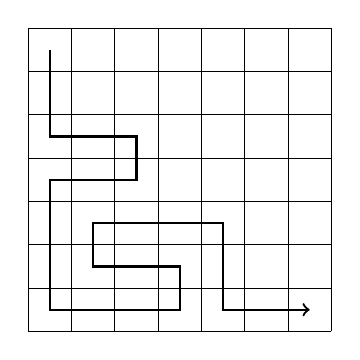
\begin{tikzpicture}[scale=.55]
  \begin{scope}
    \draw (0, 0) grid (7, 7);
    \draw[thick,->] (0.5,6.5) -- (0.5,4.5) -- (2.5,4.5) --
          (2.5,3.5) -- (0.5,3.5) -- (0.5,0.5) --
          (3.5,0.5) -- (3.5,1.5) -- (1.5,1.5) --
          (1.5,2.5) -- (4.5,2.5) -- (4.5,0.5) --
          (6.5,0.5);
  \end{scope}
\end{tikzpicture}
\end{center}
利用这个观察，如果过早到达右下角的方格，
我们可以立即终止搜索。
\begin{itemize}
\item
运行时间：119秒
\item
递归调用次数：200亿次
\end{itemize}

\subsubsection{优化3}

如果路径碰到墙壁，
并且可以向左或向右转，
则网格被分割成两个
包含未访问方格的部分。
例如，在以下情况中，
路径可以向左或向右转：

\begin{center}
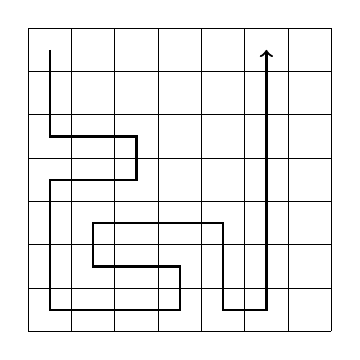
\begin{tikzpicture}[scale=.55]
  \begin{scope}
    \draw (0, 0) grid (7, 7);
    \draw[thick,->] (0.5,6.5) -- (0.5,4.5) -- (2.5,4.5) --
          (2.5,3.5) -- (0.5,3.5) -- (0.5,0.5) --
          (3.5,0.5) -- (3.5,1.5) -- (1.5,1.5) --
          (1.5,2.5) -- (4.5,2.5) -- (4.5,0.5) --
          (5.5,0.5) -- (5.5,6.5);
  \end{scope}
\end{tikzpicture}
\end{center}
在这种情况下，我们已经无法访问所有方格，
因此可以终止搜索。
这个优化非常有用：

\begin{itemize}
\item
运行时间：1.8秒
\item
递归调用次数：2.21亿次
\end{itemize}

\subsubsection{优化4}

优化3的思想
可以推广：
如果路径无法继续向前
但可以向左或向右转，
则网格被分割成两个
都包含未访问方格的部分。
例如，考虑以下路径：

\begin{center}
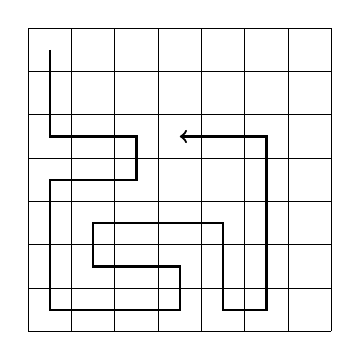
\begin{tikzpicture}[scale=.55]
  \begin{scope}
    \draw (0, 0) grid (7, 7);
    \draw[thick,->] (0.5,6.5) -- (0.5,4.5) -- (2.5,4.5) --
          (2.5,3.5) -- (0.5,3.5) -- (0.5,0.5) --
          (3.5,0.5) -- (3.5,1.5) -- (1.5,1.5) --
          (1.5,2.5) -- (4.5,2.5) -- (4.5,0.5) --
          (5.5,0.5) -- (5.5,4.5) -- (3.5,4.5);
  \end{scope}
\end{tikzpicture}
\end{center}
显然我们已经无法访问所有方格，
因此可以终止搜索。
经过这次优化后，搜索变得
非常高效：

\begin{itemize}
\item
运行时间：0.6秒
\item
递归调用次数：6900万次
\end{itemize}

~\\
现在是停止优化算法并
看看我们取得了什么成果的好时机。
原始算法的运行时间
为483秒，
而经过优化后，
运行时间仅为0.6秒。
因此，算法经过优化后
快了近1000倍。

这是回溯中的常见现象，
因为搜索树通常很大，
即使是简单的观察也能有效地
剪枝搜索。
特别是在算法的最初几步
（即搜索树的顶部）发生的优化
尤其有用。

\section{折半搜索}

\index{折半搜索}

\key{折半搜索}（Meet in the middle）是一种
将搜索空间分成
大小大致相等的两部分的
技术。
对两部分分别进行搜索，
最后将搜索结果合并。

如果有高效的方法可以合并
搜索结果，
则可以使用该技术。
在这种情况下，两次搜索可能
比一次大搜索所需的时间更少。
通常，使用折半搜索技术
可以将$2^n$的因子
转化为$2^{n/2}$的因子。

作为一个例子，考虑这样一个问题：
给定一个包含$n$个数的列表和
一个数$x$，
我们想找出是否可以从列表中选择一些数
使得它们的和为$x$。
例如，给定列表$[2,4,5,9]$和$x=15$，
我们可以选择数字$[2,4,9]$，因为$2+4+9=15$。
然而，如果对同一个列表$x=10$，
则不可能组成该和。

解决这个问题的一个简单算法是
遍历所有元素子集，
检查是否有任何子集的和为$x$。
这种算法的运行时间为$O(2^n)$，
因为有$2^n$个子集。
然而，使用折半搜索技术，
我们可以实现更高效的$O(2^{n/2})$时间算法\footnote{这个
思想由 E. Horowitz 和 S. Sahni 于1974年提出 \cite{hor74}。}。
注意，$O(2^n)$和$O(2^{n/2})$
是不同的复杂度，因为$2^{n/2}$等于$\sqrt{2^n}$。

其思想是将列表分成
两个列表$A$和$B$，使得两个
列表各包含大约一半的数。
第一次搜索生成$A$的所有子集，
并将其和存储到列表$S_A$中。
相应地，第二次搜索从$B$创建
列表$S_B$。
之后，只需检查是否可以从$S_A$中选择一个元素
以及从$S_B$中选择另一个元素，
使得它们的和为$x$。
当且仅当有一种方法可以使用原始列表中的数
组成和$x$时，这是可能的。

例如，假设列表为$[2,4,5,9]$且$x=15$。
首先，我们将列表分为$A=[2,4]$和$B=[5,9]$。
之后，我们创建列表
$S_A=[0,2,4,6]$和$S_B=[0,5,9,14]$。
在这种情况下，和$x=15$是可以组成的，
因为$S_A$包含和$6$，
$S_B$包含和$9$，且$6+9=15$。
这对应于解$[2,4,9]$。

我们可以这样实现算法，
使其时间复杂度为$O(2^{n/2})$。
首先，我们生成\emph{有序的}列表$S_A$和$S_B$，
这可以在$O(2^{n/2})$时间内使用类似归并的技术完成。
之后，由于列表是有序的，
我们可以在$O(2^{n/2})$时间内检查
是否可以从$S_A$和$S_B$创建和$x$。